\documentclass[11pt]{article}
\usepackage{lmodern}
\usepackage{amssymb,amsmath}
\usepackage{ifxetex,ifluatex}
\usepackage{fixltx2e} % provides \textsubscript
\ifnum 0\ifxetex 1\fi\ifluatex 1\fi=0 % if pdftex
  \usepackage[T1]{fontenc}
  \usepackage[utf8]{inputenc}
\else % if luatex or xelatex
  \ifxetex
    \usepackage{mathspec}
  \else
    \usepackage{fontspec}
  \fi
  \defaultfontfeatures{Ligatures=TeX,Scale=MatchLowercase}
\fi
% use upquote if available, for straight quotes in verbatim environments
\IfFileExists{upquote.sty}{\usepackage{upquote}}{}
% use microtype if available
\IfFileExists{microtype.sty}{%
\usepackage{microtype}
\UseMicrotypeSet[protrusion]{basicmath} % disable protrusion for tt fonts
}{}
\usepackage[margin=1in]{geometry}
\usepackage{hyperref}
\hypersetup{unicode=true,
            pdftitle={My Titled},
            pdfauthor={Andreas Lillevang Bech},
            pdfkeywords={Machine Learning, Big Data, Return Prediction, Cross-Section of Returns},
            pdfborder={0 0 0},
            breaklinks=true}
\urlstyle{same}  % don't use monospace font for urls
\usepackage{color}
\usepackage{fancyvrb}
\newcommand{\VerbBar}{|}
\newcommand{\VERB}{\Verb[commandchars=\\\{\}]}
\DefineVerbatimEnvironment{Highlighting}{Verbatim}{commandchars=\\\{\}}
% Add ',fontsize=\small' for more characters per line
\usepackage{framed}
\definecolor{shadecolor}{RGB}{248,248,248}
\newenvironment{Shaded}{\begin{snugshade}}{\end{snugshade}}
\newcommand{\AlertTok}[1]{\textcolor[rgb]{0.94,0.16,0.16}{#1}}
\newcommand{\AnnotationTok}[1]{\textcolor[rgb]{0.56,0.35,0.01}{\textbf{\textit{#1}}}}
\newcommand{\AttributeTok}[1]{\textcolor[rgb]{0.77,0.63,0.00}{#1}}
\newcommand{\BaseNTok}[1]{\textcolor[rgb]{0.00,0.00,0.81}{#1}}
\newcommand{\BuiltInTok}[1]{#1}
\newcommand{\CharTok}[1]{\textcolor[rgb]{0.31,0.60,0.02}{#1}}
\newcommand{\CommentTok}[1]{\textcolor[rgb]{0.56,0.35,0.01}{\textit{#1}}}
\newcommand{\CommentVarTok}[1]{\textcolor[rgb]{0.56,0.35,0.01}{\textbf{\textit{#1}}}}
\newcommand{\ConstantTok}[1]{\textcolor[rgb]{0.00,0.00,0.00}{#1}}
\newcommand{\ControlFlowTok}[1]{\textcolor[rgb]{0.13,0.29,0.53}{\textbf{#1}}}
\newcommand{\DataTypeTok}[1]{\textcolor[rgb]{0.13,0.29,0.53}{#1}}
\newcommand{\DecValTok}[1]{\textcolor[rgb]{0.00,0.00,0.81}{#1}}
\newcommand{\DocumentationTok}[1]{\textcolor[rgb]{0.56,0.35,0.01}{\textbf{\textit{#1}}}}
\newcommand{\ErrorTok}[1]{\textcolor[rgb]{0.64,0.00,0.00}{\textbf{#1}}}
\newcommand{\ExtensionTok}[1]{#1}
\newcommand{\FloatTok}[1]{\textcolor[rgb]{0.00,0.00,0.81}{#1}}
\newcommand{\FunctionTok}[1]{\textcolor[rgb]{0.00,0.00,0.00}{#1}}
\newcommand{\ImportTok}[1]{#1}
\newcommand{\InformationTok}[1]{\textcolor[rgb]{0.56,0.35,0.01}{\textbf{\textit{#1}}}}
\newcommand{\KeywordTok}[1]{\textcolor[rgb]{0.13,0.29,0.53}{\textbf{#1}}}
\newcommand{\NormalTok}[1]{#1}
\newcommand{\OperatorTok}[1]{\textcolor[rgb]{0.81,0.36,0.00}{\textbf{#1}}}
\newcommand{\OtherTok}[1]{\textcolor[rgb]{0.56,0.35,0.01}{#1}}
\newcommand{\PreprocessorTok}[1]{\textcolor[rgb]{0.56,0.35,0.01}{\textit{#1}}}
\newcommand{\RegionMarkerTok}[1]{#1}
\newcommand{\SpecialCharTok}[1]{\textcolor[rgb]{0.00,0.00,0.00}{#1}}
\newcommand{\SpecialStringTok}[1]{\textcolor[rgb]{0.31,0.60,0.02}{#1}}
\newcommand{\StringTok}[1]{\textcolor[rgb]{0.31,0.60,0.02}{#1}}
\newcommand{\VariableTok}[1]{\textcolor[rgb]{0.00,0.00,0.00}{#1}}
\newcommand{\VerbatimStringTok}[1]{\textcolor[rgb]{0.31,0.60,0.02}{#1}}
\newcommand{\WarningTok}[1]{\textcolor[rgb]{0.56,0.35,0.01}{\textbf{\textit{#1}}}}
\usepackage{graphicx,grffile}
\makeatletter
\def\maxwidth{\ifdim\Gin@nat@width>\linewidth\linewidth\else\Gin@nat@width\fi}
\def\maxheight{\ifdim\Gin@nat@height>\textheight\textheight\else\Gin@nat@height\fi}
\makeatother
% Scale images if necessary, so that they will not overflow the page
% margins by default, and it is still possible to overwrite the defaults
% using explicit options in \includegraphics[width, height, ...]{}
\setkeys{Gin}{width=\maxwidth,height=\maxheight,keepaspectratio}
\IfFileExists{parskip.sty}{%
\usepackage{parskip}
}{% else
\setlength{\parindent}{0pt}
\setlength{\parskip}{6pt plus 2pt minus 1pt}
}
\setlength{\emergencystretch}{3em}  % prevent overfull lines
\providecommand{\tightlist}{%
  \setlength{\itemsep}{0pt}\setlength{\parskip}{0pt}}
\setcounter{secnumdepth}{5}
% Redefines (sub)paragraphs to behave more like sections
\ifx\paragraph\undefined\else
\let\oldparagraph\paragraph
\renewcommand{\paragraph}[1]{\oldparagraph{#1}\mbox{}}
\fi
\ifx\subparagraph\undefined\else
\let\oldsubparagraph\subparagraph
\renewcommand{\subparagraph}[1]{\oldsubparagraph{#1}\mbox{}}
\fi

%%% Use protect on footnotes to avoid problems with footnotes in titles
\let\rmarkdownfootnote\footnote%
\def\footnote{\protect\rmarkdownfootnote}

%%% Change title format to be more compact
\usepackage{titling}

% Create subtitle command for use in maketitle
\providecommand{\subtitle}[1]{
  \posttitle{
    \begin{center}\large#1\end{center}
    }
}

\setlength{\droptitle}{-2em}

  \title{Robustness of Machine Learning in \protect\\
  Empirical Asset Pricing}
    \pretitle{\vspace{\droptitle}\centering\huge}
  \posttitle{\par}
    \author{Andreas Lillevang Bech}
    \preauthor{\centering\large\emph}
  \postauthor{\par}
      \predate{\centering\large\emph}
  \postdate{\par}
    \date{June 2019}

%Preamble for ETE memo
\usepackage{amsmath}
\usepackage{graphicx}
\usepackage{threeparttable}
\usepackage[capposition=top]{floatrow}
\usepackage{makecell}
\newcommand{\sgn}{\mathrm{sgn}}
\usepackage{booktabs}
\usepackage{longtable}
\usepackage{array}
\usepackage{multirow}
\usepackage{wrapfig}
\usepackage{float}
\usepackage{colortbl}
\usepackage{pdflscape}
\usepackage{tabu}
\usepackage{threeparttable}
\usepackage{threeparttablex}
\usepackage[normalem]{ulem}
\usepackage{makecell}
\usepackage{xcolor}
\usepackage{algorithm}
\usepackage[noend]{algpseudocode}
\usepackage{bm}
\linespread{1.1}


\makeatletter
\def\BState{\State\hskip-\ALG@thistlm}
\makeatother

\begin{document}
\maketitle
%\begin{abstract}
%\end{abstract}

\hypertarget{introduction}{%
\section{Introduction}\label{introduction}}

This paper revolves around replicating Gu, Kelly, and Xiu (2018) in
which the return predictability of financial assets is explored. A
catalog of Machine Learning methods are evaluated on their relative
performance out-of-sample on varying time horizons and data generating processes.
The comparisons are done by a simulation study, where the true data generating processes are known, and in an empirical study using data from the S\&P500 index and various macroeconomic variables as predictors.

The paper is structured as follows. A theoretical section introduces the
statistical models under evaluation, as well as the validation approach used for
choosing between model specifications. Then the simulation study and its results are presented. Finally the methods are tested in the empirical example.

\hypertarget{theoretical-section}{%
\section{Theoretical section}\label{theoretical-section}}

\hypertarget{statistical-model}{%
\subsection{Statistical Model}\label{statistical-model}}

The model most often considered in the context of statistical learning
is the additive error model.

\[r_{i,t+1} = E_t(r_{i,t+1}) + \epsilon_{t+1}\] where
\[E_t(r_{i,t+1}) = g(z_{i,t})\]

The conditional expectation, which is the aim of the estimation
procedure, is a function of the available predictors at time t,
\(z_{i,t}\). In almost any statistical setting, a pair \((r_{i,t+1},z_{i,t})\)
will not have a deterministic relationship of the form
\(r_{i,t+1} = E_t(r_{i,t+1})\). Therefore an additive error,
\(\epsilon_{t+1}\), is usually added to give a complete characterization
of the truth\footnote{See Friedman, Hastie, and Tibshirani (2001)}.

The difference in this setting, as compared to the usual cross-sectional
machine learning framework, is the time component. The data in this
setting is a panel of stocks, each stock indexed by i and the time
period by t. Thus predictors at time t of stock i, \(z_{i,t}\), may
include past observations of the response or predictor variables, e.g.
recent price trends like reversal and momentum\footnote{Which may or may
not be proxies for time-varying beta compensation Kelly, Moskowitz,
and Pruitt (2018)}. This adds some considerations for the estimation
procedure. The conditional expectation is a function of the predictors
\(z_{i,t}\) and here it is denoted \(g\). \(g\) is assumed to have the
same form across time and individual stocks, which gives in all
\(N\times T\) observations for estimation. \(T\) is the number of
time periods and \(N\) is the number of individual stocks. As
there is a time order to the observations that should be preserved, the sample-splitting procedure will be slightly restricted.

\hypertarget{tuning-parameters-hyper-parameters}{%
\subsection{Tuning parameters (hyper
parameters)}\label{tuning-parameters-hyper-parameters}}

Machine learning models have so-called tuning parameters which usually
qualify the degree of complexity of the models, i.e.~how much they try
to adapt to a given set of training data. Examples of tuning parameters
are the penalty parameter in Lasso estimation, the no. of knots and
degrees in a piece wise polynomial function, or the depth of a
regression tree. As the training error always decreases with more
complexity, a ``validation'' procedure is needed to restrict the model.
Validation amounts to estimating the test error in order to choose the
degree of complexity in a given model that performs best for
forecasting/prediction.

Due to the time element in the data, which we wish to conserve in
chronological order (some predictor variables like momentum use the past
returns), cross-validation is not appropriate for choosing tuning
parameters. Instead, sample-splitting, dividing the training data into a
\emph{training} and a \emph{validation} part will allow to evaluate an
estimated model on new data while still keeping the test data locked up
for final evaluation. Choosing tuning parameters simply amounts to
choosing the model that performs best in the validation sample. The
following pseudo code illustrates the idea.

\begin{Shaded}
\begin{Highlighting}[]
\CommentTok{# split data}
\NormalTok{data =}\StringTok{ }\NormalTok{...}
\NormalTok{train, validation, test =}\StringTok{ }\KeywordTok{split}\NormalTok{(data)}

\CommentTok{# tune model hyperparameters}
\NormalTok{parameters =}\StringTok{ }\NormalTok{...}
\ControlFlowTok{for}\NormalTok{ params }\ControlFlowTok{in}\NormalTok{ parameters}\OperatorTok{:}
\StringTok{    }\NormalTok{model =}\StringTok{ }\KeywordTok{fit}\NormalTok{(train, params)}
\NormalTok{    skill =}\StringTok{ }\KeywordTok{evaluate}\NormalTok{(model, validation)}

\CommentTok{# evaluate final model for comparison with other models}
\NormalTok{model =}\StringTok{ }\KeywordTok{fit}\NormalTok{(train)}
\NormalTok{skill =}\StringTok{ }\KeywordTok{evaluate}\NormalTok{(model, test)}
\end{Highlighting}
\end{Shaded}

\hypertarget{linear-models}{%
\subsection{Linear models}\label{linear-models}}

Linear regression is a model based approach which imposes that the
conditional expectation is linear in its arguments \(f(x) = x'\theta\).

The \textbf{simple linear model} is where each predictor enters as an
argument as it is, \(g(z_{i,t}) =z_{i,t}' \theta\). The
parameters, \(\theta\), of the model can be estimated using the training
data, most popularly by \emph{least squares} which chooses the parameters
to minimize the objective function of the residual sum of squares

\[RSS(\theta) = \sum_{i=1}^N\sum_{t=1}^T (r_{i,t+1} - g(z_{i,t};\theta) )^2\]
Here there are \(T\times N\) observations as the pooled estimate of
\(\theta\) over the panel of individual stocks is considered.

It is well known that the linear model has a low bias. However, in the
face of a large amount of predictors relative to number of observations,
the linear model will have large variance. In this context, as Gu,
Kelly, and Xiu (2018) points out, what really matters is the number of
predictors \(p\) vs.~time periods \(T\), as stock returns typically
share a large cross-sectional dependence which limits the information
gained by adding observations along the cross-section.

\hypertarget{penalized-regression}{%
\subsubsection{Penalized Regression}\label{penalized-regression}}

Although there are variable subset select procedures that can be
performed even on large models, like Forward- and Backward-Stepwise
selection\footnote{see Friedman, Hastie, and Tibshirani (2001), chapter
  3.3}, a more efficient way to reduce the complexity of the linear
model is to impose constraint on the size (norm) of \(\theta\). This is done
via a penalty in the objective function, such that parameters are
estimated by minimizing

\[
\mathcal{L}(\theta,\cdot) = RSS(\theta) + \phi(\theta, \cdot)
\] where the penalty function \(\phi\) depends on a tuning parameter.

For \textbf{Ridge regression} an L2 penalty is applied to the
parameters. In this case
\(\phi(\theta, \lambda) = \lambda \|\theta \|_2^2\) such that the
parameters are constrained in a hypersphere in the parameter space with
center at the origin. Shrinking the parameters in this way introduces
bias to the linear model but can be shown to reduce the variance. In
terms of expected prediction error this often leads to better out of
sample predictions in high dimensional problems.

Another proposed way of shrinking the parameters is with an L1 penalty,
\(\phi(\theta, \lambda) = \lambda \|\theta \|_1\). Regression with this
penalty is known as \textbf{Lasso regression}. Geometrically this means
that the parameters are constrained in a ``diamond'' (L1 unit circle),
which will tend to set many parameters to exactly zero and thus working
as actual subset selection of the variables. This is opposed to the
Ridge regression that will never set parameters to zero.\footnote{see
  again Friedman, Hastie, and Tibshirani (2001), chapter 3.3, for a
  visual illustration of the difference between Ridge and Lasso penalty.}.

Finally a combination of the two approaches to the penalty has been
proposed by Zou and Hastie (2005), known as the \textbf{Elastic Net}. It
uses a linear combination between the penalties,
\(\phi(\theta, \lambda, \alpha) = \lambda \left( \alpha \|\theta \|_2^2 + (1-\alpha) \|\theta \|_1 \right)\).
For \(\alpha < 1\) the constraint boundary still has ``kinks'' at
\(\theta_j = 0\) and thus still enjoys the property of the Lasso of
deselecting some variables.

The \textbf{implementation} of penalized regression is not always straightforward. In this case, stack the available panel data in a matrix with one observation in each row and call it \textbf{X}. And call the \(NT\) response vector \textbf{y}. The Ridge regression solutions are well defined and unique as the objetive function, \(\mathcal{L}(\theta,\lambda)\), is strictly convex and continuously differentiable. They are easily seen to be 

\[
\hat{\beta}_{\lambda}^{Ridge} = \big( \lambda \bm{I_P} + 
\frac{1}{NT} \bm{X'X} \big)^{-1} \frac{1}{NT} \bm{X'y}
\]

and, in fact, \( \big( \lambda \bm{I_P} + \frac{1}{NT} \bm{X'X} \big) \) is always positive definite as long as \(\lambda\) is positive.

However, the same does not go for the Lasso and the Elastic Net, and to these there exists no closed form solutions. To compute the Lasso and Elastic Net coefficients one can use the Least Angle Regression (LAR) algorithm introduced by Efron et al., (2004) and the slightly modified version (LARS-EN) introduced by Zou and Hastie (2005). The LARS algorithm is detailed below. It can be shown that the LAR path is equal to the Lasso path as the penalty parameter is moved towards zero. 

\begin{algorithm}
  \caption{Least Angle Regression}
  \begin{algorithmic}[1]
  \State z-standardize predictors and initialize from residual $r = y - \bar{y}$ and $\beta_1, \beta_2, \dots, \beta_p = 0$
  \State Find predictor $x_j$ most correlated with r.
  \State Increase $\beta_j$ in the direction of $sign(corr(r, xj ))$ until another predictor $x_k$ has an equal absolute correlation with current residual as $x_j$.
  \State Move ``active'' variables' coefficient towards joint least squares coefficients of the current residuals on the active set until another variable cathes up in terms of correlation.
  \State Continue until all variables are included, which gives the least squares estimates.
\end{algorithmic}
\end{algorithm}

\hypertarget{pcr-and-plsr}{%
\subsubsection{PCR and PLSR}\label{pcr-and-plsr}}

Principal Components Regression and Partial Least Squares Regression are
linear models that consider certain linear combinations of the
predictors and use these as arguments in the linear model. Such methods
are derived to reduce the dimension of the problem, which is especially
useful if there are a large number of highly correlated predictors. The
two methods differ in how they utilize the inputs.

\textbf{PCR} seeks to use as much variation from the inputs in as few
variables as possible. It does this by using the principal components of
the input data. The largest principal component is the direction in the
input space that yields the largest variance if all input point where
projected onto this line. Call a vector point in this direction
\(\bm{v_1} \in \mathbb{R}^p\), then the first/largest principal component is
\(\bm{X v_1}\). The second principal component maximizes this variance
subject to being orthogonal to \(v_1\). There are in total \(P\)
principal components and the choice of how many to include in the linear
model as arguments is a tuning parameter subject to validation.

To find the principal components of the centered input matrix one can use \emph{singular value decomposition},

\[
\bm{X = UDV'}  
\]

where \(\bm{U}\) and \(\bm{V}\) are \( NT \times p \) and \( p \times p \) orthogonal matrices with the columns of \(\bm{U}\) spanning the column space of \(\bm{X}\) and the columns of \(\bm{V}\) spanning the row space of \(\bm{X}\). \(\bm{D}\) is a diagonal matrix and the entries are called the \emph{singular values} of \(\bm{X}\). It is seen clearly that the eigendecomposition of the sample covariance of the inputs is given by

\[
  \bm{X'X = VD^2V'}
\]

And thus the columns of \(\bm{V}\) are the eigenvectors of the sample covariance and these are exactly the principal components of \(\bm{X}\). Principal component regression with \(M\) components is then just a linear model with arguements \(\bm{z_1, z_2}, \dots, \bm{z_M}\) where \(\bm{z_j} = \bm{Xv_j}\) and \(M<P\).

The second approach, \textbf{PLSR}, instead tries to maximize the
covariance with the responses (returns). In essence the first argument,
the first partial squares direction, put forward to the model is a
weighted sum of the predictors where predictors (after having been
standardized) with higher covariance with the response have higher
weights. To include more directions the inputs are orthogonalized wrt. the first direction and the procedure is repeated again. How many arguments to give the model is again a tuning paramenter.

Thus the derived inputs for PLSR stem from inputs' covariance with the response. Implementation of PLSR is straightforward, and is presented in algorithm 2.

\begin{algorithm}
  \caption{Partial Least Squares}
  \begin{algorithmic}[2]
  \State z-standardize predictors and initialize from $\hat{y}^{(0)} = \bar{y}\bm{1}$ and $\bm{x}_j^{(0)} = \bm{x}_j, \textrm{  } j = 1, \dots, P$
  \State For $m = 1, \dots, P$ \newline
  (a) $\bm{z_m} = \sum_{j=1}^P \hat{\phi}_{mj} \bm{x}_j^{(m-1)}, \textrm{ where } \hat{\phi}_{mj} = \langle \bm{x}_j^{(m-1)}, \bm{y} \rangle $ \newline
  (b) As $z_m$'s are orthogonal the partial linear coefficient is the simple linear coefficient $\hat{\theta}_m = \frac{\langle \bm{z_m}, \bm{y} \rangle}{\langle \bm{z_m}, \bm{z_m} \rangle}$ \newline
  (c) $\hat{y}^{(m)} = \hat{y}^{(m-1)} + \hat{\theta}_m \bm{z_m}$ \newline
  (d) orthogonalize each $\bm{x}_j^{(m-1)}$ with respect to $\bm{z_m}$ 
  \end{algorithmic}
\end{algorithm}


\hypertarget{generalized-linear-model}{%
\subsubsection{Generalized Linear
Model}\label{generalized-linear-model}}

The final linear model considered in this exercise is the \textbf{GLM}.
Each predictor is transformed by a \emph{linear basis expansion} and a
linear model is then fit in this new space of derived inputs. Because the
basis functions most often are non-linear, such a model can capture
non-linearities in the data as the regression function/surface
\(f(x)\) is non-linear. However the model is still linear in the
coefficients to be estimated which is why such a model is also referred to
as ``additive''.

In this exercise a second order spline expansion is chosen, as is done in Gu,
Kelly, and Xiu (2018). A quadratic spline is a piecewise/local second
order polynomial that is restricted to be continuous and
have a continuous first derivatives at the ``knots''. Having restricted
the local polynomials to be quadratic, the only tuning parameter is the
no. of knots, more knots leading to a more complex model.

As the number of parameters in such a model is much greater than in the
simple linear model it is surely advantageous to use a shrinking method.
In this setting the Group Lasso is useful. It gives the following penalty to the
objective function

\[\phi(\theta, \lambda, K) = \lambda \sum_{j=1}^P \left(  \sum_{k=1}^K \theta_{j,k}^2   \right)^{1/2}\]

where P is the no. of predictors available and K is the no. of terms in
a given spline considered. The Group Lasso penalty has the desirable
property that terms based on the same predictor are set to zero
together. Thus for the GLM considered here, the no. of knots and the
penalty parameter, \(\lambda\), are the tuning parameters.

\hypertarget{tree-based-models}{%
\subsection{Tree-based Models}\label{tree-based-models}}

Tree regression takes a completely different approach to approximating the
conditional expectation of the response given the inputs,
\(f(x) = E[Y|X=x]\). Instead of using a continuous surface over the
predictor space the approach is instead to divide the predictor space
into rectangles and treat \(f(x)\) as constant in each rectangle. This
is a very direct approach to approximate \(E[Y|X=x]\), where the
(empirical) mean is conditioned not at the point \(x\) but in on an area
around \(x\). The size of each rectangle is what determines the
complexity of a tree regression.

To find the optimal division of the predictor space by considering all
options is computationally infeasible. The most common procedure is a
\emph{greedy} one where at each step the space or a ``branch'' of the
space is split by a predictor and a split value, both of which are
chosen to reduce the RSS maximally for that step. Each split creates two
new branches. This procedure known as \emph{recursive binary splitting}.

Splitting/branching halts when the tree reaches a prespecified stopping
criterion. In this paper the stopping criterion is based on a minimal
no. of observations in each terminal node (``leaf'') or reach of a depth
limit, both are chosen as tuning parameters based on the validation
sample.

Unlike the GLM where individual predictors can predict in a non-linear
fashion, regression trees allow for more flexible non-linear effects,
particularly in the form interactions between variables. A tree divides
the p-dimensional input space into (hyper)rectangles which allows for
interactions for up to all p predictors. A regression tree, however,
suffers from high variance in the sense that a small perturbation in the
input values can lead to a large change in a given tree. This amounts to
easily overfitting on the training data. The variance issue of trees has
been very successfully addressed by forecasting based on averaging over
many trees, a method known as ensemble learning. Two ways of this approach are considered, ``boosting'' and ``bagging''.

Boosting fits an oversimplified/``shallow'' tree on the training data
and then fits a consecutive tree on the residuals from the first tree.
Then the sum of the forecasts for the two trees is considered as the
forecast, but where the second tree's forecast (of the residuals) is
shrunk by a factor between \(\nu \in (0,1)\). A third tree is added to
these residuals and so on.. This approach is commonly known as \textbf{Gradient Boosted Regression Trees} (GBRT) Tuning parameters to be chosen are the limit
depth of each tree, the shrinkage factor and the total number of trees
to fit. For boosting a maximal of 6 splits is typically considered,
hence the ``slow learning'' approach.

For bagging, many trees are fitted using (nonparametric-)bootstrap
samples and then averaged. To avoid using the most influential variables
for the first splits in all the trees, only a random subset of the
predictors are considered for splitting at each branch. This amounts to
a \textbf{Random Forest}. The Random Forest is fairly straightforward to
use ``out-of-the-box'' and performs very well without having a lot of
tuning parameters to be chosen. The most important tuning parameter is
the fraction of predictors available for each split. The number of trees
should be chosen but the MSE will stabilize after a while. The node size
should also be chosen, as a stopping criterion, which also represents a
bias-variance trade-off as smaller nodes will lead to more complex
trees.

For \textbf{Implementaion} of either method the build of a regression tree will be the same. Using recursive binary splitting. Starting from the top, a splitting variable \(\bm{x}_j\) and a splitting point \(s\) divides the input space into two half-spaces

\[
R_1(j,s) = \{X|X_j < s\} \quad \textrm{and} \quad R_2(j,s) = \{X|X_j > s\}    
\]

The problem is then to find a pair \((j,s)\) that solves the problem

\[
\min_{j,s}  [ \min_{c_1} \sum_{x_i \in R_1(j,s)} (y_i - c_1) + \min_{c_2} \sum_{x_i \in R_2(j,s)} (y_i - c_2)  ]  
\]

where the inner minimization problem solutions, \(\hat{c}_1\) and \(\hat{c}_2\), are solved by the average of the responses associated to an input in the given region, \(R\). An exhaustive search is used and is very fast. To implement the GBRT method follow the steps in algorithm 3.

\begin{algorithm}
  \caption{Gradient  Boosted Regression Trees}
  \begin{algorithmic}[3]
  \State Set $\hat{f}(x) = 0$ and $r_i = y_i$ for each training example $i$.
  \State For $ b = 1, \dots, B$ \newline
  (a) Fit a tree $\hat{f}^b$ on $r$ with the chosen stopping criterion \newline
  (b) Update the model by adding a shrunking version of the new tree $\hat{f}(x) = \hat{f}(x) + \nu \hat{f}^b(x) $ \newline
  (c) Update the residuals $r_i = y_i - \hat{f}(x)$ \newline
  \State Output the model $\hat{f}(x)$  
  \end{algorithmic}
\end{algorithm}

\newpage

\hypertarget{neural-networks}{%
\subsection{Neural Networks}\label{neural-networks}}

\begin{wrapfigure}{R}{0.5\textwidth}
    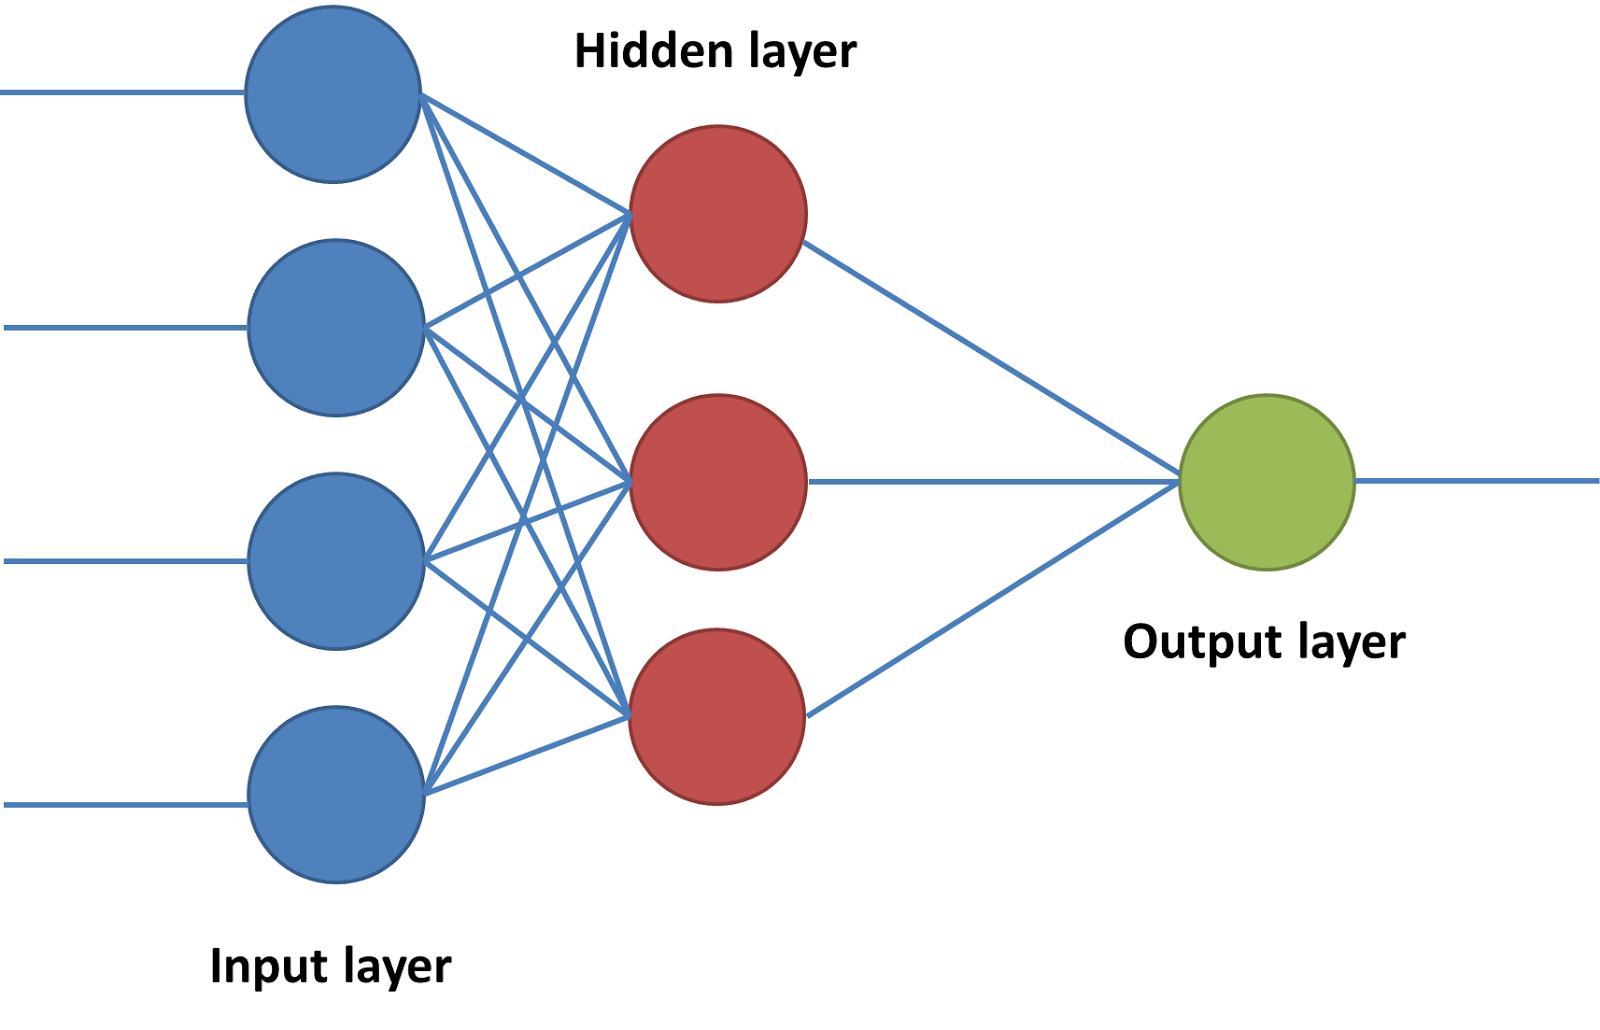
\includegraphics[width=0.90\textwidth]{/Users/alexanderbech/dropbox/project/iu.png}
  \caption{Illustration of simple Feed-forward Neural Network}
\end{wrapfigure}

The final learning method considered, which is in a category of its own,
is the \textbf{Neural Network} (NN). The inputs are filtered through
``hidden layers'' to create new arguments to use as predictors in a
linear model. This is analogous to PCR and PLSR, however, the neural
network is not as systematic and is much more flexible. Figure 1 gives a
simple illustration of a Neural Network in the regression context. There
are 4 input/predictors and one hidden layer with 3 ``neurons''. Each
neuron gets its value as a linear combination of all the neurons from the
previous layer. Without any hidden layer this is just a simple linear
regression.

The NN allows for non-linear regression by applying a non-linear
``activation function'' to each neuron in the hidden layers. In fact a
NN with just a single hidden layer containing a finite number of neurons
can approximate continuous functions on compact subsets of
\(\mathbb{R}^n\) (see Cybenko 1989). The NN's in this exercise uses the
ReLU activation function \(ReLU(x) = \max\{x,0\}\). The NN's flexibility
is also one of its greatest criticisms and it is often described as a
``black box'' without any meaning, just pure pattern recognition.

For the number of parameters in a neural network, consider a NN with one
hidden layer, with, say, \(n\) neurons. There are \(p\) predictors, thus
each neuron in the hidden layer has to it associated (p+1) parameters
(it's a linear model in itself). This gives \(n \times(p+1)\) parameters
in the hidden layer. Additionally, there will be \((n+1)\) parameters in
the output layer which constitute the linear model for predicting the
output with the neurons from the hidden layer. In all
\(n \times(p+1) + (n+1)\) parameters in the neural network with one
hidden layer containing \(n\) neurons. The large number of parameters
are obviously a problem for contexts with few observations for
estimation, like in the context of economics and finance. Thus in these
contexts shallow networks with few neurons in each layer tend to perform
better.

In this exercise NN's with layers ranging from 1-3 are considered, and
the no. of neurons in each layer is set by the geometric pyramid rule
(see Masters 1993). In estimation RSS is used as an objective. It is
optimized by Stochastic Gradient Descent (SGD) and an l1 penalty on the
parameters is used to prevent overfitting - this is also called ``weight
decay''. Another measure against overfitting is ``early stopping'' which
evaluates the error on a validation sample after each epoch in the SGD. If
the validation error increases for 3 epochs in a row the fitting is
stopped. Important tuning parameters are the parameter penalties and the
step size in the SGD.

\textbf{Fitting} a Neural Network with SGD is often termed \emph{back-propagation}. If we let \(w_{jk}\) denote the matrix parameters\footnote{j refers to the jth neuron in layer l while k refers to the kth neuron in the previous layer, layer (l-1)}, or \emph{weights} as they will be called from here, in a given layer of a NN, gradient descent updates the weights by the negative gradient for each step in the optimization

\[
  w_{jk} \rightarrow w_{jk}' = w_{jk} - \eta \frac{\partial \mathcal{L}}{\partial w_{jk}}
\]
for each \((j,k)\). Here \(\eta \) is the step size/learning rate and \(\mathcal{L}\) is the loss function which here is assumed to be the RSS

\[
  \mathcal{L}(w) = \sum_{i=1}^N (y_i - f(x_i))^2
\]

"Stochastic" refers to the fact that not the whole training sample is used in each iteration, but instead a random subsample (a "batch") of the training sample. The gradient computed with the subsample can be understood as an approximation of the actual gradient and is used to significantly speed up the procedure.

The term back-propagation comes form the computation of the gradient of the loss function. For a NN with one hidden layer we need the partial derivatives of the weights in the hidden layer, \(\frac{\partial \mathcal{L}}{\partial w_{jk}}\), where \(w_{jk}\) is a matrix of weights connecting the kth input to the jth neuron. We also need the partial derivatives of the weights in the final output layer, \(\frac{\partial \mathcal{L}}{\partial \beta_{j}}\). 

Thus, if \(z_j\) refers to the activated jth neuron in the hidden layer, \(f(x) = \beta_0 + \beta'z\) while \(z_j = \sigma(w_{0j} + \sum_k w_{jk}x_k)\), where \(\sigma\) refers to the activation function. A simple use of the chain rule then gives the partial derivatives for a training example \(i\)

\begin{align*}
  \frac{\partial \mathcal{L}_i}{\partial \beta_{j}} &= -2(y_i - f(x_i))z_{ji} \\
  \frac{\partial \mathcal{L}_i}{\partial w_{jk}} &= -2(y_i - f(x_i))\beta_{j}\sigma'(w_0j + \sum_k w_{jk}x_{ki})x_{ki}
\end{align*}

The \(\sigma\) activation function is not always differentiable, like the ReLU used here is not differentiable at \(0\). However, this does not have great importance for the optimization and nothing is lost by setting the derivative at \(0\) equal to \(0\).

A useful concept is the \emph{error} of the ith training example, \(\delta_i\), and the partial derivatives are usually written like this

\begin{align*}
  \frac{\partial \mathcal{L}_i}{\partial \beta_{j}} &= \delta_i z_{ji} \\
  \frac{\partial \mathcal{L}_i}{\partial w_{jk}} &= \delta_i \beta_{j}\sigma'(w_0j + \sum_k w_{jk}x_{ki})x_{ki}
\end{align*}

The term back-propagation comes from the fact that the algorithm works in two passes. First, for a given set of weights, a training example is fed to the model which gives the error, \(\delta_i\). From then it is straightforward to calculate the gradient as all of \(x_{ki}, z_{ji}, \beta_j, w_{jk}, \sigma'\) are known. Then the weights are nudged with the given step size, \(\eta\), which concludes an iteration. 

The procedure is repeated until a given stopping criterion is met, in this case early stopping, as described above.

\hypertarget{evaluation}{%
\subsection{Evaluation}\label{evaluation}}

In this paper model performance is based on the R-squared measure. Both
for in-sample and out-of-sample the RSS is compared to the total sum of
squares based on the historical mean of the returns, i.e the average of
returns before the test sample. Out-of-sample R-squared is then

\[
R^2_{OOS} = 1 - \frac{\sum_{(i,t)\in\mathrm{test}} (r_{i,t+1} - \hat{r}_{i,t+1} )^2}{\sum_{(i,t)\in\mathrm{test}} (r_{i,t+1}- \bar{r}_{train})^2 }
\] Models can be compared pairwise for their out-of-sample predictive
ability by the Diebold-Mariano test\footnote{Diebold and Mariano (2002)}.
The test considers the difference in errors from two different models

\[d_t = \left(e_{i,t}^{(1)}\right)^2 - \left(e_{i,t}^{(2)}\right)^2\]

where errors \(e_{i,t}\) are transformed with the square - the absolute
value could also be used\footnote{When doing the test on a panel it makes
  to average prediction error for each model in each time period,
  i.e.~in the cross-section. This is due to the high error dependence
  across stocks, which likely violates the conditions for asymptotic
  normality of the test statistic.}. Under the null hypothesis both
model perfrom equally well, \(\bar{d}= 0\) and the limiting distribution
is

\[\sqrt{T}\bar{d} \xrightarrow[]{d} N\left(0, \sum_{k=-\infty}^{\infty} \gamma_d(k)\right)\]

given that this second moment is bounded. Here \(\gamma_d(k)\) is the autocovariance of \(d_t\) at k lags. The long run variance of the sample mean is\footnote{see Hamilton (1995)}

\[\mathrm{Var}(\sqrt{T}\bar{d}) \xrightarrow[]{T\rightarrow \infty} \sum_{k=-\infty}^{\infty} \gamma_d(k)\]

Thus test statistics will be

\[\frac{\bar{d}}{\sqrt{ \frac{\sum_{k=-\infty}^{\infty} \gamma_d(k)}{T}  }}\]

which is asymptotically standard normal. The HAC estimator proposed by
Newey and West (1987) is used to get a consistent estimate of the
variance.

\hypertarget{simulation}{%
\section{Simulation}\label{simulation}}

\hypertarget{data-generating-process}{%
\subsection{Data Generating Process}\label{data-generating-process}}

The simulation is based on the experiment outlined in Gu, Kelly, and Xiu
(2018). The experiment is set up to compare model performance for
different data generating processes.\footnote{I will give the outline of
  the experiment. The specifics can be found in the appendix of Gu,
  Kelly, and Xiu (2018) under the name ``Monte Carlo simulations''.}

DGP-a is a linear DGP such that returns in the following period for
individual stock i is a linear combination of three of the respectively
100 and 200 available predictors. To the extent that machine learning
models is thought to capture non-linearities among the predictors, the
simple linear model (OLS)\footnote{Here and in the rest of the paper OLS
  is meant to be the naive linear model of all predictors entering
  without transformations. No variable selection is performed. Other
  linear models considered in the simulation study are the penalty
  methods of Ridge, Lasso and Elastic net, and the Generalized Linear
  Model (Generalized Additive Model) where splines of variables are
  used. The oracle is the linear model where only the true predictors
  from the DGP enter} should perform relatively well in this. A
different number of total predictors for each stock is considered to
evaluate the improvement shrinking and dimensionality reductions methods
can provide.

The other DGP considered, DGP-b, is a non-linear counterpart. The same
predictors enter the true DGP in the construction of returns/responses,
however, each variable enters as a non linear transformation.

Specifically the setup is like this. The returns are made up by the
conditional expectation, g, given the predictors, plus an error.

\[r_{i,t+1}= g(z_{i,t}) + e_{i, t+1}\] \(e_{i, t+1}\) is a combination
of a normal error and a student error, it is common to both
DGP's\footnote{see the appendix of Gu, Kelly, and Xiu (2018) for details.}.

Choosing the data generating process is choosing g. The set of
predictors for each stock i, \(z_{i,t}\) is made up of individual
characteristics, \(c_{i,t}\), and interactions of the characteristics
with a common macroeconomic variable, \(x_t\). That is,
\(z_{i,t} = (1, x_t)' \otimes c_{i,t}\). If there are \(Pc\) individual
characteristics there will thus be \(P = 2 \times Pc\) predictors for
each individual stock \(i\) at time \(t\). The individual
characteristics are generated using an AR(1) process with normal error
and with AR-coefficient randomly distributed uniform(0.9, 1), such that
there is a high degree of persistence in the characteristics. The
macroeconomic variable, \(x_t\), is similarly generated as an AR(1) with
normal error and AR-coefficient \( = 0.95\).

\[
\begin{aligned}
(a) & = g(z_{i,t}) =  (c_{i1,t}, c_{i2,t}, c_{i3,t} \times x_t)\theta_0, \quad \mathrm{where} \quad \theta_0 = (0.2, 0.2, 0.2)'   \\
(b) & = g(z_{i,t}) = \big(c_{i1,t}^2, c_{i1,t} \times c_{i2,t}, \sgn(c_{i3,t} \times x_t) \big)\theta_0, \quad \mathrm{where} \quad \theta_0 = (0.04, 0.03, 0.012)' 
\end{aligned}
\]

\hypertarget{results}{%
\subsection{Results}\label{results}}

Due to a computing power issue a slight deviation from the simulation
study in Gu, Kelly, and Xiu (2018) is that the number of firms (N) is
100 instead of 200 and the number of periods (T) is 90 instead of 180.
It is not clear in the paper whether or not an expanding window with
recursive estimation is considered in the simulation study. Due to the
computing power issue a fixed window is used here, where only one
estimation is needed for each simulation repetition. This decision
should not have a large impact as the DGP remains the same over time
in the simulated data.

The linear models to be compared are pooled OLS, Ridge, Lasso and
Elastic Net (ENET). OLS is the naive approach where variable selection
is not performed. Further the more complex linear models of Principal
Component regression (PCR), Partial Least Squares regression (PLSR) and
the Generalized Linear/Additive model (GLM) are also estimated on each
simulated data. For the tree based methods, Gradient Boosted regression
trees (GBRT) and Random Forest are considered. Finally Neural Networks
(NN) with 1-3 layers are estimated.

\begin{table}[ht]
\begin{threeparttable}
\centering
\setlength{\tabcolsep}{12pt}
\caption{Comparison of Predictive $R^2$s for Machine Learning Algorithms in Simulations}
\begin{tabular}{lrrrrcrrrr}
DGP & \multicolumn{4}{c}{(a)} && \multicolumn{4}{c}{(b)} \\
  \Xhline{2\arrayrulewidth}\noalign{\smallskip}
Parameter & \multicolumn{2}{c}{$P_c = 50$} & \multicolumn{2}{c}{$P_c = 100$}& & \multicolumn{2}{c}{$P_c = 50$} &  \multicolumn{2}{c}{$P_c = 100$} \\
  \noalign{\smallskip}\hline\noalign{\smallskip}
$R^2(\%)$ & \multicolumn{1}{c}{IS} & \multicolumn{1}{c}{OOS} & \multicolumn{1}{c}{IS} & \multicolumn{1}{c}{OOS} & &\multicolumn{1}{c}{IS} & \multicolumn{1}{c}{OOS} & \multicolumn{1}{c}{IS} & \multicolumn{1}{c}{OOS} \\ 
  \noalign{\smallskip}\hline\noalign{\smallskip}
OLS & 10.11 & -1.30 & 12.90 & -3.79 && 6.87 & -5.73 & 9.45 & -8.82 \\ 
Ridge & 8.06 & 1.47 & 9.35 & 1.01 && 4.56 & -0.19 & 5.54 & -0.15 \\ 
Lasso & 8.12 & 2.61 & 9.37 & 1.86 && 4.54 & -0.43 & 5.60 & -0.03 \\ 
ENet & 8.18 & 2.69 & 9.53 & 1.89 && 4.66 & -0.41 & 5.72 & -0.07 \\ 
PCR & 7.46 & 0.08 & 8.32 & -0.04 && 4.23 & -0.68 & 4.97 & -0.72 \\ 
PLSR & 7.38 & 0.27 & 8.51 & -0.16 && 3.67 & -1.98 & 4.50 & -3.36 \\ 
GLM & 7.92 & 0.21 & 9.07 & 0.01 && 4.80 & -0.48 & 5.87 & -0.98 \\ 
RandomF & 13.91 & 2.33 & 16.39 & 1.83 && 13.49 & 1.02 & 14.74 & 2.23 \\ 
GBRT & 9.84 & 1.94 & 11.59 & 0.55 && 10.06 & 1.09 & 10.37 & 1.20 \\ 
NN1 & -6.42 & 1.60 & -26.00 & -15.46 && -10.43 & -0.70 & -11.44 & -1.21 \\ 
NN2 & -12.41 & 1.67 & -13.49 & 1.05 && -13.26 & -0.05 & -15.26 & -0.04 \\ 
Oracle & 8.41 & 3.45 & 10.04 & 3.74 && 4.89 & 0.12 & 5.81 & -0.07 \\ 
   \Xhline{2\arrayrulewidth}
\end{tabular}
\begin{tablenotes}
      \small
      \item Note: The table report in-sample (IS) and out-of-sample (OOS) $R^2$s for the different data generating processes (a) and (b). The forecasting methods use are OLS using all available varialbles, Ridge, Lasso, Elastic Net (ENet), Principal Component Analysis (PCR), Partial Least Squares (PLSR), Random Forest, Gradient Boosted Tree Regression (GBRT), and Neural Networks with 1-3 layers (NN). The Oracle is a linear model using only variables present in the true DGP. N=100, T=90 and Pc considered are 50 and 100. The number of Monte Carlo repetitions is 50.
    \end{tablenotes}
  \end{threeparttable}
\label{table:simulation}
\end{table}

The results of the simulation study can be found in Table 1, which presents the \(R^2\)'s. In the appendix, Tables 5-8 present Diebold Mariano tests for pairwise comparisons. A remark: the Neural Networks with 3 layers were not trained correctly as some did not converge, at all, to a minimum, and therefore these
are not present in the table. The Neural Networks with 1 and 2 layers do not perform as well as in the paper by Gu, Kelly, and Xiu (2018), and there might be a problem with the training algorithm used.

In terms of replicating Gu, Kelly, and Xiu (2018) it is mostly a
positive result. For the linear DGP, (a), the Ridge and Elastic net
regressions perform very well. This is unsurprising as these are linear
models with shrinking and variable selection, allowing them to come
potentially close in model specification to the true process. The
dimension reduction methods, like PCR and PLSR, do not perform as well.
Likely due to the very low signal-to-noise ratio in this kind of data.
The very complex and adaptive linear model, GLM, does not perform well
either, and probably for the same reason. The GLM has a lot of variables
to estimate in a linear regression and thus suffers from high variance.
The tree based regressions perform as well as the best linear ones, even
though the DGP is completely linear. This goes in particular for the
Random Forest. 

For DGP (a) and 50 individual characteristics, \(P_c = 50 \), it is however only the Oracle which performs significantly better than any of the other models. For \(P_c = 100 \) there is more significance. Lasso, Elastic Net, Random Forest and the Oracle all perform significantly better than OLS. Furthermore, Elastic Net performs significantly better than both PCR and PLSR. See Tables 5 and 6 in the appendix.

The more interesting finding is to be made for the non-linear DGP, (b).
Recall that in this case the returns are constructed by the square of an
input, an interaction between two inputs and the sign function of an
input, which is of course not continuous. Now almost all models perform
worse than the historical average by having a negative \(R^2\)
out-of-sample. The only models to perform with a positive \(R^2\) are
the tree based models. This is in line with Gu, Kelly, and Xiu (2018)
and points towads these models, \emph{homogeneous} ensembles of trees,
as being very effective in high noise environments. In fact, GBRT and
Random Forests perform even better with \(P_c=100\) than for \(P_c=50\),
i.e.~with more noise, both here and in the paper by Gu, Kelly, and Xiu
(2018).

For DGP (a) and 50 individual characteristics, Random Forest, GBRT and the Oracle perform significantly better than OLS, and Random Forest and GBRT perform better than PLSR as well. With 100 characteristics the Lasso and Elastic Net significantly outperform other models too, both OLS and PLSR, indicating sparsity is valuable.

\begin{table}[ht]
\begin{threeparttable}
\centering
\setlength{\tabcolsep}{5pt}
\caption{Comparison of Predictive $R^2$s for Machine Learning Algorithms in Simulations}
\begin{tabular}{lrrrrrrcrrrrrr}
DGP & \multicolumn{6}{c}{(a)} && \multicolumn{6}{c}{(b)} \\
  \Xhline{2\arrayrulewidth}\noalign{\smallskip}
Horizon & \multicolumn{2}{c}{Quarter} & \multicolumn{2}{c}{Halfyear} & \multicolumn{2}{c}{Annual} && \multicolumn{2}{c}{Quarter} & \multicolumn{2}{c}{Halfyear} & \multicolumn{2}{c}{Annual} \\ 
   \noalign{\smallskip}\hline\noalign{\smallskip}
$R^2(\%)$ & \multicolumn{1}{c}{IS} & \multicolumn{1}{c}{OOS} & \multicolumn{1}{c}{IS} & \multicolumn{1}{c}{OOS} &\multicolumn{1}{c}{IS} & \multicolumn{1}{c}{OOS} && \multicolumn{1}{c}{IS} & \multicolumn{1}{c}{OOS} &\multicolumn{1}{c}{IS} & \multicolumn{1}{c}{OOS} & \multicolumn{1}{c}{IS} & \multicolumn{1}{c}{OOS}\\ 
  \noalign{\smallskip}\hline\noalign{\smallskip}
OLS & 22.45 & -5.49 & 29.91 & -16.92 & 44.61 & -10.61 && 15.30 & -20.43 & 25.37 & -28.22 & 33.69 & -44.38 \\ 
Ridge & 14.39 & 2.81 & 18.02 & 1.08 & 29.24 & 5.54 && 6.01 & -0.63 & 12.00 & -0.48 & 15.44 & -4.27 \\ 
Lasso & 14.27 & 6.00 & 17.20 & 7.88 & 27.92 & 14.84 && 5.20 & 0.09 & 11.09 & -0.28 & 11.81 & -2.86 \\ 
ENet & 14.52 & 6.11 & 17.76 & 8.03 & 28.40 & 14.86 && 6.09 & -0.42 & 11.87 & -0.10 & 14.65 & -4.26 \\ 
PCR & 11.98 & 0.23 & 15.31 & -5.32 & 22.99 & 0.94 && 3.94 & -1.13 & 9.84 & -1.30 & 11.61 & -5.16 \\ 
PLSR & 11.63 & 0.94 & 12.05 & -4.45 & 27.24 & -1.61 && 6.41 & -7.93 & 9.72 & -8.70 & 13.72 & -20.01 \\ 
GLM & 13.46 & 0.30 & 17.54 & -4.13 & 29.03 & 0.12 && 6.76 & -2.44 & 10.12 & -2.43 & 11.77 & -6.03 \\ 
RandomF & 88.03 & 6.64 & 91.13 & 10.27 & 94.29 & 20.30 && 87.51 & 4.70 & 91.34 & 7.58 & 93.72 & 10.04 \\ 
GBRT & 17.84 & 5.99 & 21.89 & 7.67 & 36.57 & 12.07 && 15.67 & 2.51 & 22.53 & 2.90 & 30.81 & -1.57 \\ 
NN1 & 6.68 & 5.22 & -0.38 & -21.73 & 23.42 & -61.45 && 0.23 & -4.55 & -3.66 & -34.08 & 9.07 & -71.39 \\ 
Oracle & 15.33 & 8.91 & 18.72 & 10.93 & 28.75 & 20.59 && 6.30 & -0.48 & 11.48 & -0.48 & 11.46 & -1.25 \\ 
  \Xhline{2\arrayrulewidth}
\end{tabular}
\begin{tablenotes}
      \small
      \item Note: The table reports in-sample (IS) and out-of-sample (OOS) $R^2$s for the different data generating processes (a) and (b) and longer horizons. That is 3 months, 6 months and 12 months. The data frequency is monthly. The forecasting methods use are OLS using all available varialbles, Ridge, Lasso, Elastic Net (ENet), Principal Component Analysis (PCR), Partial Least Squares (PLSR), Random Forest, Gradient Boosted Tree Regression (GBRT), and Neural Networks with 1-3 layers (NN). The Oracle is a linear model using only variables present in the true DGP. N=100, T=90 and P=100. The number of Monte Carlo repetitions is 50.
    \end{tablenotes}
  \end{threeparttable}
\label{table:horizon}
\end{table}

Table 2 explores the relative performance of the different methods over
longer horizons. For DGP (a), as compared to 1-period out-of-sample,
performance is \emph{better} for models that performed well in 1-period
forecasts, but \emph{worse} for models that performed poorly before. As
an example, the shrinkage and selection methods of Lasso and Elastic
Net, which performed well for the linear DGP, (a), perform even better
on longer horizons. For the annual horizon these models explain almost
15\% of the out-of-sample variation. Likewise, the tree based
regressions perform better the longer the horizon with the Random Forest
being able to explain 20\% of the variation of the linear process one
year out of sample. In contrast, the poorer models perform similarly or
worse on longer horizons. The Neural Network performs extremely bad on
long horizons meaning that it fails to pick up on the essential part of
the DGP, i.e. it recognizes a complex pattern that is not relevant to the DGP.

For the non-linaer DGP, (b), all models perform worse, expect for the
Random Forest. It seems that longer horizons does not aid in finding the
true DGP despite the underlying variables, the characteristics, being
generated as mean-reverting processes (AR(1)'s). This does not go,
however, for the Random Forest, which performs better the longer the
horizon. An explanation for this is that the trees used in Random Forest
are complex and thus has the ability to pick up on a non-linear,
discontinuous pattern, while still avoiding overfitting with the use of
bagging.

\hypertarget{empirical-exercise}{%
\section{Empirical Exercise}\label{empirical-exercise}}


\begin{figure}[ht]
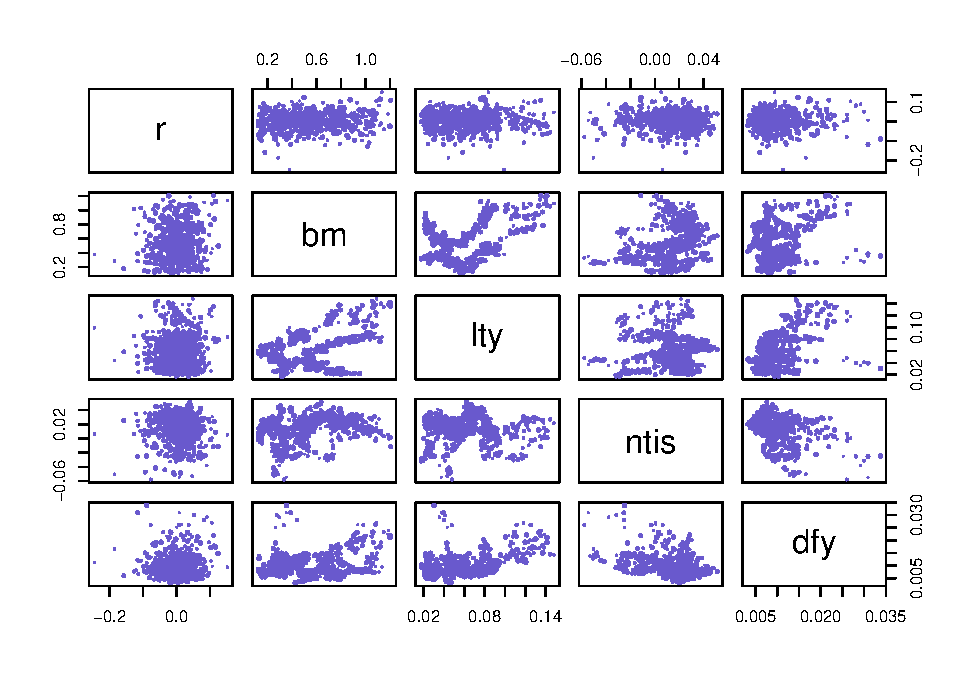
\includegraphics[width=0.75\linewidth]{mark_files/figure-latex/unnamed-chunk-2-1} \caption{Scatterplot-matrix for the data from @goyalwelch2008}\label{fig:unnamed-chunk-2}
\floatfoot{Note: \textbf{r} is log returns on the S\&P500, \textbf{bm} is the ratio
of book value to market value for the Dow Jones Industrial Average,
\textbf{lty} are the Long-term government bond yields from Ibbotson's
Stocks, Bonds, Bills and Inflation Yearbook\footnote{See Stocks (1995)},
\textbf{ntis} is the ratio of twelve-month moving sums of net issues by
NYSE listed stocks divided by the total market capitalization of NYSE
stocks and finally \textbf{dfy} the default yield spread is the
difference between BAA- and AAA- rated cor- porate bond yields.}
\end{figure}

Given data compiled for the paper Welch and Goyal (2008)\footnote{The
  data, including an appendix with sources and description of the data,
  can be found on Amit Goyal's website
  \url{http://www.hec.unil.ch/agoyal/}}. The sample considered runs from
1947-03-01 to 2017-06-01. The data is monthly in frequency but some
variables are only updated on a quarterly or annual basis. Index is the
S\&P500 without dividends.

The data is divided into training, validation and test samples. The
training sample runs in 1947-1982, 35 years, the validation sample in
(1982-2000), 18 years, and finally the test sample the final 17 years.

The crucial difference between the data used in the paper Gu, Kelly, and
Xiu (2018, 2018) and the data collected here is the number of
observations. In the data from Welch and Goyal (2008) only returns on
the stock market index (S\&P500) is considered as the response. Thus,
the only relevant predictors are aggregated macroeconomic
characteristics from the stock market including dividend-price ratio
(dp), earnings-price ratio (ep), book-to-market ratio (bm), net equity
expansion (ntis), Treasury-bill rate (tbl), term spread (tms), default
spread (dfy), and stock variance (svar). In Gu, Kelly, and Xiu (2018)
data are obtained at an individual stock level and with stock individual
characteristics. Predictors such as growth in common shareholder equity and gross
profitability are therefore available. This gives more
observations as well as more predictors, which in turn gives a more
stable estimation and more information to forecast with. Nevertheless, it is an interesting exercise to see how the different machine learning
models compare in the case considered here (with no cross-section).

A scatterplot matrix of the data, Figure 2, shows well the small
correlation between the log returns and the predictors. Included are the log returns as well as the 4 most relevant predictors in
terms of significance in correlation. Looking at the top row it is clear
that there is very little ``signal'' to extract form the data, at least
from linear dependence.

\begin{table}[ht]
\begin{threeparttable}
\centering
\setlength{\tabcolsep}{6pt}
\caption{Comparison of Predictive $R^2$s for Machine Learning Algorithms in Simulations}
\begin{tabular}{rrrrrrrrrrrrr}
  \Xhline{2\arrayrulewidth}
 & OLS & Ridge & Lasso & ENet & PCR & PLSR & GLM & RandomF & GBRT\\ 
  \hline
OOS & -21.60 & 1.22 & -2.51 & -3.16 & -7.21 & -13.55 & -19.95 & -9.59 & -3.60 \\
IS & 9.29 & 3.70 & 3.69 & 3.70 & 4.70 & -1.08 & 3.69 & 12.42 & 9.89  \\ 
   \Xhline{2\arrayrulewidth}
\end{tabular}
\begin{tablenotes}
      \small
      \item Note: Model performance on the data from Welch and Goyal (2008). Neural Networks are excluded as they did not come to a reasonable estimate. Data can be found at Amit Goyal's website http://www.hec.unil.ch/agoyal/.
    \end{tablenotes}
  \end{threeparttable}
\label{table:data}
\end{table}

Table 3 gives the performance of the models on the empirical data.
Out-of-sample all models perform worse than the historical average,
except the Rigde regression which performs slightly better. Comparing
the in-sample forecasts the Ridge has among the highest error, which
indicates that the Ridge does well not to overfit on the data. This
property is useful in an environment with not many observations to train
on and very little signal in each observation. The tree based
regressions which performed very well in the simulations perform
significantly worse now, with the Random Forest being among the poorest
out-of-sample predictors.

Model performance can be tested pairwise by the Diebold Mariano test.
The quadradic error is used in the test which puts more emphasis
on big errors in prediction. The absolute value or even non-symmetric
transformations of errors are other options. Table 4 gives the results
of the tests. Bold font indicates a significant difference at the 5\%
level and a positive number indicates the column model outperforms the
row model.

\begin{table}[ht]
\begin{threeparttable}
\centering
\setlength{\tabcolsep}{5pt}
\caption{Comparison of Monthly Out-of-Sample Prediction using Diebold-Mariano Tests}
\centering
\begin{tabular}{r|rrrrrrrr}
  \Xhline{2\arrayrulewidth}
 & Ridge & Lasso & ENET & PCR & PLSR & GLM & RandomF & GBRT \\ 
  \hline
OLS & \textbf{2.40} & \textbf{2.03} & 1.95 & 1.64 & 0.63 & 0.10 & 1.95 & 1.93 \\ 
  Ridge && -1.57 & -1.84 & \textbf{-1.97} & -1.78 & -1.62 & \textbf{-2.59} & -0.89 \\ 
  Lasso &&& \textbf{-2.18} & \textbf{-2.11} & -1.46 & -1.27 & -1.59 & 0.28 \\ 
  ENET &&&& -1.79 & -1.41 & -1.22 & -1.44 & 0.51 \\ 
  PCR &&&&& -0.80 & -0.85 & -0.38 & 1.44 \\ 
  PLSR  &&&&&& -0.38 & 0.53 & 1.43 \\ 
  GLM  &&&&&&& 0.85 & 1.23 \\ 
  RandomF  &&&&&&&& 1.33 \\ 
   \Xhline{2\arrayrulewidth}
\end{tabular}
\begin{tablenotes}
      \small
      \item Note: This table reports pairwise Diebold-Mariano test statistics comparing the out-of-sample prediction performance among nine models. Positive numbers indicate the column model outperforms the row model. Bold font indicates the difference is significant at 5\% level or better.
    \end{tablenotes}
  \end{threeparttable}
\label{table:diebold}
\end{table}

To explore how the models are chosen across time, Figure 3 graphs model complexity based on particular criteria for each model. For the Lasso and Elastic net choosing more
parameters to be non-zero amounts to more complexity. For PCR and PLSR
the no. of directions is chosen as a measure. For the GRBT the chosen
tree depth is plotted. Finally for the Random Forest the minimum
terminal node size is plotted. Note that the Random Forest is opposite
in terms of complexity as larger node size means a less complex tree.

There is a bit of a tendency for the model complexity to decrease over
time. An explanation for this could be that the ``information''
available in the market has decreased as more of the computational
techniques have become more widely available.

\begin{figure}[H]
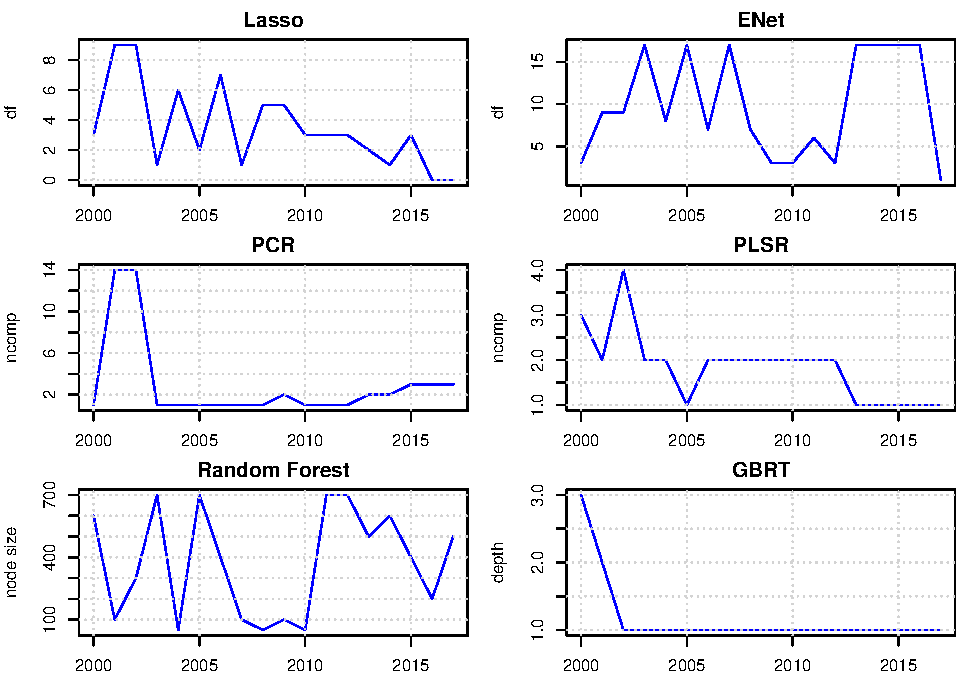
\includegraphics[width=0.75\linewidth]{mark_files/figure-latex/complexity_plots-1} \caption{Model complexity over time}\label{fig:complexity_plots}
\floatfoot{Note: This figure demonstrates the model complexity over time for Lasso,
Elastic net (ENet), PCR, PLS, Random Forest (RF) and Gradient Boosted
Regression Trees (GBRT) in each training sample of the 18-year recursive
out-of-sample analysis. For ENet and Lasso the number of variables
selected to have non-zero coefficients are reported; for PCR and PLS
reported is the number of selected components/directions; for RF
reported is the tuned minimal node size; and for GBRT the tuned tree
depth.}
\end{figure}

\hypertarget{conclusion}{%
\section{Conclusion}\label{conclusion}}

The main finding in this paper is that Machine Learning methods can pose
an important tool in empirical asset pricing and financial/economic
forecasting. Both simpler methods like Lasso regression and more
advanced techniques like Random Forests provide more stable methods for
forecasting, even in high noise data, than the standard linear model. The Lasso improves on the linear model by shrinking and selecting parameters in a continuous way by
adding a penalty to the objective function. This improves on the linear models
variability, even on the linear model with variable selection (see
Friedman, Hastie, and Tibshirani 2001, vol. 1, chap. 3.4). Random
Forest presents a complete alternative method to the linear model by
using tree regression for the conditional expectation. Together with the
gradient boosted tree regression, these methods are the standout
performers in this high noise environment, especially with the
non-linear data generating process.

There is an ambiguity, however. In the empirical study, where much fewer observations were available, the Random Forest fails to perform well out-of-sample. The Ridge regression on the other hand, which was not a stand-out performer anywhere in the simulation study, performed well and was the only model to outperform the historical average.

\hypertarget{references}{%
\section{References}\label{references}}

\hypertarget{refs}{}
\leavevmode\hypertarget{ref-cybenko1989approximations}{}%
Cybenko, George. 1989. ``Approximations by Superpositions of a Sigmoidal
Function.'' \emph{Mathematics of Control, Signals and Systems} 2:
183--92.

\leavevmode\hypertarget{ref-diebold2002comparing}{}%
Diebold, Francis X, and Robert S Mariano. 2002. ``Comparing Predictive
Accuracy.'' \emph{Journal of Business \& Economic Statistics} 20 (1).
Taylor \& Francis: 134--44.

\leavevmode\hypertarget{ref-friedman2001elements}{}%
Friedman, Jerome, Trevor Hastie, and Robert Tibshirani. 2001. \emph{The
Elements of Statistical Learning}. Vol. 1. 10. Springer series in
statistics New York.

\leavevmode\hypertarget{ref-NBERw25398}{}%
Gu, Shihao, Bryan Kelly, and Dacheng Xiu. 2018. ``Empirical Asset
Pricing via Machine Learning.'' Working Paper 25398. Working Paper
Series. National Bureau of Economic Research.
\url{https://doi.org/10.3386/w25398}.

\leavevmode\hypertarget{ref-hamilton1995time}{}%
Hamilton, James D. 1995. \emph{Time Series Analysis}. \emph{Economic
Theory. II, Princeton University Press, USA}.

\leavevmode\hypertarget{ref-james2013introduction}{}%
James, Gareth, Daniela Witten, Trevor Hastie, and Robert Tibshirani.
2013. \emph{An Introduction to Statistical Learning}. Vol. 112.
Springer.

\leavevmode\hypertarget{ref-kelly2018understanding}{}%
Kelly, Bryan T, Tobias J Moskowitz, and Seth Pruitt. 2018.
``Understanding Momentum and Reversal.'' \emph{Available at SSRN
3269897}.

\leavevmode\hypertarget{ref-masters1993practical}{}%
Masters, Timothy. 1993. \emph{Practical Neural Network Recipes in C++}.
Morgan Kaufmann.

\leavevmode\hypertarget{ref-neweywest1987}{}%
Newey, Whitney K., and Kenneth D. West. 1987. ``A Simple, Positive
Semi-Definite, Heteroskedasticity and Autocorrelation Consistent
Covariance Matrix.'' \emph{Econometrica} 55 (3). {[}Wiley, Econometric
Society{]}: 703--8. \url{http://www.jstor.org/stable/1913610}.

\leavevmode\hypertarget{ref-stocks1995bills}{}%
Stocks, Bonds. 1995. ``Bills and Inflation 1995 Yearbook.''
\emph{Ibbotson Associates, Chicago}.

\leavevmode\hypertarget{ref-goyalwelch2008}{}%
Welch, Ivo, and Amit Goyal. 2008. ``A Comprehensive Look at the
Empirical Performance of Equity Premium Prediction.'' \emph{The Review
of Financial Studies} 21 (4). {[}Oxford University Press, Society for
Financial Studies{]}: 1455--1508.
\url{http://www.jstor.org/stable/40056859}.

\leavevmode\hypertarget{ref-zou2005regularization}{}%
Zou, Hui, and Trevor Hastie. 2005. ``Regularization and Variable
Selection via the Elastic Net.'' \emph{Journal of the Royal Statistical
Society: Series B (Statistical Methodology)} 67 (2). Wiley Online
Library: 301--20.

\leavevmode\hypertarget{ref-zou2005regularization}{}%
Efron, Bradley, Trevor Hastie, Iain Johnstone, and Robert Tibshirani. ``Least angle regression.'' \emph{The Annals of statistics} 32, no. 2 (2004): 407-499.

\newpage

\hypertarget{appendix}{%
\section{Appendix}\label{appendix}}

\begin{table}[H]
\begin{threeparttable}
\centering
\setlength{\tabcolsep}{5pt}
\caption{Comparison of Out-of-Sample Prediction in the Simulation study using Diebold-Mariano Tests. DGP (a), Pc=50.}
\centering
\begin{tabular}{r|rrrrrrrrrr}
  \Xhline{2\arrayrulewidth}
& Ridge & Lasso & ENET & PCR & PLSR & GLM & RandomF & GBRT & Oracle \\ 
  \hline
OLS & 0.72 & 1.31 & 1.33 & 0.05 & 0.39 & 0.40 & 1.14 & 1.17 & \textbf{2.26} \\ 
  Ridge  && 0.92 & 0.88 & -1.08 & -0.37 & -0.48 & 0.50 & 0.58 & 1.17 \\ 
  Lasso  &&& 0.21 & -1.31 & -1.00 & -0.87 & -0.06 & -0.14 & 0.60 \\ 
  ENET  &&&& -1.49 & -1.05 & -1.02 & -0.05 & -0.19 & 0.60 \\ 
  PCR  &&&&& 0.71 & 0.30 & 1.15 & 1.10 & 1.51 \\ 
  PLSR  &&&&&& -0.15 & 0.77 & 0.87 & 1.44 \\ 
  GLM &&&&&&& 0.74 & 0.73 & 1.20 \\ 
  RandomF  &&&&&&&& 0.06 & 0.91 \\ 
  GBRT &&&&&&&&& 0.70 \\ 
   \Xhline{2\arrayrulewidth}
\end{tabular}
\begin{tablenotes}
      \small
      \item Note: This table reports pairwise Diebold-Mariano test statistics comparing the out-of-sample prediction performance among ten models. Positive numbers indicate the column model outperforms the row model. Bold font indicates the difference is significant at 5\% level or better. DGP (a), Pc=50.
    \end{tablenotes}
  \end{threeparttable}
\label{table:dieboldsim1}
\end{table}

%%%%%%%%%%%%%%%%%%%

\begin{table}[H]
\begin{threeparttable}
\centering
\setlength{\tabcolsep}{5pt}
\caption{Comparison of Out-of-Sample Prediction in the Simulation study using Diebold-Mariano Tests. DGP (a), Pc=100.}
\centering
\begin{tabular}{r|rrrrrrrrrr}
  \Xhline{2\arrayrulewidth}
& Ridge & Lasso & ENET & PCR & PLSR & GLM & RandomF & GBRT & Oracle \\ 
  \hline
OLS  & 1.15 & \textbf{2.06} & \textbf{2.08} & 0.73 & 0.81 & 0.89 & \textbf{1.98} & 1.79 & \textbf{2.78} \\ 
  Ridge  && 1.49 & 1.61 & -1.15 & -0.93 & -0.01 & 0.94 & 1.02 & 1.37 \\ 
  Lasso &&& 0.28 & -1.87 & \textbf{-2.17} & -1.42 & -0.28 & -0.56 & 0.76 \\ 
  ENET  &&&& \textbf{-1.96} & \textbf{-2.20} & -1.44 & -0.29 & -0.59 & 0.74 \\ 
  PCR  &&&&& 0.20 & 0.62 & 1.37 & 1.29 & 1.74 \\ 
  PLSR  &&&&&& 0.40 & 1.53 & 1.75 & 2.01 \\ 
  GLM &&&&&&& 1.03 & 0.90 & 1.61 \\ 
  RandomF  &&&&&&&& -0.13 & 1.07 \\ 
  GBRT &&&&&&&&& 0.94 \\ 
   \Xhline{2\arrayrulewidth}
\end{tabular}
\begin{tablenotes}
      \small
      \item Note: This table reports pairwise Diebold-Mariano test statistics comparing the out-of-sample prediction performance among ten models. Positive numbers indicate the column model outperforms the row model. Bold font indicates the difference is significant at 5\% level or better. DGP (a), Pc=100.
    \end{tablenotes}
  \end{threeparttable}
\label{table:dieboldsim2}
\end{table}


%%%%%%%%%%%%%%%%%%%%%%%%%%%%%


\begin{table}[H]
\begin{threeparttable}
\centering
\setlength{\tabcolsep}{5pt}
\caption{Comparison of Out-of-Sample Prediction in the Simulation study using Diebold-Mariano Tests. DGP (b), Pc=50.}
\centering
\begin{tabular}{r|rrrrrrrrrr}
  \Xhline{2\arrayrulewidth}
& Ridge & Lasso & ENET & PCR & PLSR & GLM & RandomF & GBRT & Oracle \\ 
  \hline
OLS  & 1.05 & 1.42 & 1.42 & 0.78 & 0.48 & 1.16 & \textbf{2.68} & \textbf{2.48} & \textbf{2.04} \\ 
  Ridge & & 0.35 & 0.27 & -0.69 & -0.80 & 0.23 & 1.47 & 1.77 & 0.80 \\ 
  Lasso && & -0.02 & -1.00 & -1.03 & -0.01 & 1.35 & 1.53 & 0.65 \\ 
  ENET &&& & -0.97 & -1.03 & 0.03 & 1.38 & 1.55 & 0.66 \\ 
  PCR &&&& & -0.37 & 0.78 & 1.63 & 1.86 & 1.03 \\ 
  PLSR &&&&&& 0.87 & \textbf{2.08} & \textbf{2.56} & 1.59 \\ 
  GLM&&&&&& & 1.26 & 1.33 & 0.32 \\ 
  RandomF &&&&&&& & -0.19 & -1.24 \\ 
  GBRT &&&&&&&& & -1.11 \\ 
   \Xhline{2\arrayrulewidth}
\end{tabular}
\begin{tablenotes}
      \small
      \item Note: This table reports pairwise Diebold-Mariano test statistics comparing the out-of-sample prediction performance among ten models. Positive numbers indicate the column model outperforms the row model. Bold font indicates the difference is significant at 5\% level or better. DGP (b), Pc=50.
    \end{tablenotes}
  \end{threeparttable}
\label{table:dieboldsim3}
\end{table}


%%%%%%%%%%%%%%%%%%%%%%%%%%%%%%%%%%%


\begin{table}[H]
\begin{threeparttable}
\centering
\setlength{\tabcolsep}{5pt}
\caption{Comparison of Out-of-Sample Prediction in the Simulation study using Diebold-Mariano Tests. DGP (b), Pc=100.}
\centering
\begin{tabular}{r|rrrrrrrrrr}
  \Xhline{2\arrayrulewidth}
& Ridge & Lasso & ENET & PCR & PLSR & GLM & RandomF & GBRT & Oracle \\ 
  \hline
  OLS & \textbf{2.43} & \textbf{2.78} & \textbf{2.81} & \textbf{2.29} & \textbf{1.98} & \textbf{2.28} & \textbf{4.04} & \textbf{3.48} & \textbf{3.32} \\ 
  Ridge  && 0.33 & 0.29 & -0.45 & -1.44 & 0.39 & 1.55 & 1.30 & 0.36 \\ 
  Lasso  &&& 0.18 & -0.76 & -1.67 & 0.22 & 1.51 & 1.39 & 0.21 \\ 
  ENET  &&&& -0.68 & -1.78 & 0.20 & 1.53 & 1.33 & 0.20 \\ 
  PCR  &&&&& -1.13 & 0.81 & 1.61 & 1.41 & 0.59 \\ 
  PLSR  &&&&&& 1.27 & \textbf{2.47} & \textbf{2.86} & 1.44 \\ 
  GLM  &&&&&&& 1.30 & 1.15 & 0.35 \\ 
  RandomF &&&&&&&& -0.48 & -1.44 \\ 
  GBRT  &&&&&&&&& -0.93 \\ 
   \Xhline{2\arrayrulewidth}
\end{tabular}
\begin{tablenotes}
      \small
      \item Note: This table reports pairwise Diebold-Mariano test statistics comparing the out-of-sample prediction performance among ten models. Positive numbers indicate the column model outperforms the row model. Bold font indicates the difference is significant at 5\% level or better. DGP (b), Pc=100.
    \end{tablenotes}
  \end{threeparttable}
\label{table:dieboldsim4}
\end{table}




\end{document}
